\documentclass[12pt, a4paper]{article}
\usepackage[utf8]{inputenc}

	\usepackage{graphicx, float, amssymb, wrapfig, amsthm, enumitem, amsmath, mathtools}

\graphicspath{ {pics/} }


% break style 
\newtheoremstyle{break}
{\topsep}
{\topsep}%
{\itshape}
{}%
{\bfseries}
{:}%
{\newline}
{}%

\newtheoremstyle{lemma}% style name
{2ex}% above space
{2ex}% below space
{\upshape}% body font
{}% indent amount
{\scshape}% head font
{.}% post head punctuation
{\newline}% post head punctuation
{}% head spec

%theorem styles

\theoremstyle{break}
\newtheorem{defn}{Definizione}
\AfterEndEnvironment{definizione}{\noindent\ignorespaces}


\theoremstyle{lemma}
\newtheorem{eser}{Esercizio}


\theoremstyle{lemma}
\newtheorem{dimo}{Dimostrazione}

\theoremstyle{lemma}
\newtheorem{esem}{Esempio}

% custom fraction
\newcommand*{\bfrac}[2]{\genfrac{\lbrace}{\rbrace}{0pt}{}{#1}{#2}}
\title{Appunti}
\author{Andreas Araya Osorio}
\date{3 June 2021}

\begin{document}
\maketitle
% comments can be written this way%
\section{Insiemi}

\subsection{Introduzione}

\begin{defn}
	Un insieme è una "collezione" di oggetti.
\end{defn}

Sia $A$ un \textsc{insieme}, la scrittura $ x \in A $ significa che $x \quad
appartiene \quad ad \quad A$.

Analogamento, scrivendo $ x \notin A $ si intende che $ x \quad non \quad appartiene \quad ad \quad A$.

Gli insiemi \textbf{finiti} si possono denotare all'interno di parentesi graffe $ " \{ , \} " $

Un qualsiasi insieme può definirsi mediante una \textbf{proprietà astratta}

\begin{esem}
	\begin{equation}
	A\ =\ \{\ x \in \mathbb{N}\ |\ x\ pari\ \}
	\end{equation} 
	Questo insieme raccoglie \textbf{tutti i numeri naturali pari} e si può meglio riscrivere così:
	\begin{equation}
	A\ =\ \{\ x\ \in \mathbb{N}\ |\ \exists y \in \mathbb{N}\ :\ x\ =\ 2y\ \}
	\end{equation}
\end{esem}

\subsection{Insiemi ed operazioni}
Sia $X$ un insieme e siano $A,B\ \subseteq\ X$
\begin{itemize}
	\item \textbf{UNIONE} $A \cup B$, L'unione di A e B come l'insieme 
		\begin{equation}
			A \cup B\ =\ \{ x \in X\ :\ x\in A\ o\ x\in B\ \}
		\end{equation}
	\item \textsc{INTERSEZIONE} $A \cap B$, L'intersezione di A e B come l'insieme
		\begin{equation}
			A \cap B\ =\ \{ x \in X\ :\ x\in A\ e\ x\in B\ \}
		\end{equation}
	\item \textsc{DIFFERENZA} $A \setminus B$, che equivale a
		\begin{equation}
			A \setminus B\ =\ \{x \in X\ :\ x \in A\ e\ x \notin B\ \}
		\end{equation}
	\item \textsc{COMPLEMENTARE} L'insieme complementare di $A$ in $X$ è:
		\begin{equation}
			A^C\ =\ X \setminus A\ =\ \{x \in X\ :\ x \notin A\ \}
		\end{equation}
\end{itemize}

\begin{esem}

Il complementare dell'unione è l'intersezione dei complementari, mentre il complementare dell'intersezione è l'unione dei complementari.

	\begin{itemize}
	\item $ X \setminus (A \cup B)\ =\ (X \setminus A) \cap(X \setminus B) $
	\item $ X \setminus (A \cap B)\ =\ (X \setminus A) \cup (X \setminus B) $
        \end{itemize}
\end{esem}

\begin{dimo}
	Si dice relazione da $A$ a $B$ ogni sottoinsieme $R$ di $A\times B$ Se $(a,b)\ \in\ R$.
	$a$ è in relazione $R$ con $b$, si scrive $aRb$. 
	\begin{equation} 
		\textit{R}\ = \{ (a,b) \in \mathbb{N}\ \times \mathbb{N}: \exists p \in \mathbb{N}\ |\ a\ = p \cdot b\ \}
	\end{equation}
\end{dimo}

\subsection{Relazioni d'ordine}
Sia $A\ \neq\ \varnothing$ un insieme non vuoto e sia $R\ \subseteq\ A\ \times\ A$ una relazione di $A$ con $A$. $R$ è:

\begin{enumerate}
	\item riflessiva se $xRx \quad \forall x \in A$,
	\item simmetrica se $xRy\ \rightarrow\ yRx$,
	\item transitiva se $xRy\ \land\ yRz\ \rightarrow\ xRz$,
	\item antisimmetrica se $xRy\ \land\ yRz\ \rightarrow\ x\ =\ y$.
\end{enumerate}
Una \textbf{relazione d'equivalenza} è tale se è \textsc{riflessiva, simmetrica e transitiva}.

\begin{defn} 
 	Una relazione d'ordine su un insieme $X\ \neq \ \varnothing $ è detta di  \textit{ordine totale} se $\forall\ x,y\ \in\ X $ si ha $x\ \leq\ y\ \lor\ y\ \leq\ x$. Se su $X$ c'è una relazione d'ordine totale, $X$ è totalmente ordinato. 
\end{defn}

\begin{defn} Sia $(X,\leq)$, insieme non vuoto e ordinato e sia $A \subseteq X,\ A \neq\ \varnothing$
\begin{itemize}
	\item $x \in X$ è un \textbf{maggiorante} di $A$ se $a \leq x\ \forall a\in A$
	\item $y \in X$ è un \textbf{minorante} di $A$ se $y \leq x\ \forall a\in A$
	\item $A$ ha \textbf{massimo} se $\exists \lambda \in A\ |\ a \leq \lambda\ \forall a \in A\ \implies\ \lambda\ =\ max\ A$
	\item $A$ ha \textbf{minimo} se $\exists \mu \in A\ |\ \mu \leq a\ \forall a \in A\ \implies\ \mu\ =\ min\ A$
\end{itemize}
\end{defn}

\begin{defn} Siano $(X,\leq)$ un insieme ordinato e $A\ \subseteq\ X, A\ \neq\ \varnothing$. $A$ ha \textit{estremo superiore} se l'insieme dei maggioranti di $A$ è non vuoto e ha minimo. $sup A$ è il più piccolo dei maggioranti.
Analogamente \textit{l'estremo inferiore} è presente se l'insieme dei minoranti di $A$ è non vuoto ed esso ne è il più piccolo: $inf A$.
\end{defn}

\begin{defn} \textbf{Proprietà di $sup$ e $inf$:}

		Siano $(X,\leq)$ un insieme ordinato e $A\ \subseteq\ X, A\ \neq\ \varnothing $.

                \textbf{SUP} Si ha che $\lambda\ =\ sup\ A$ \textbf{se e solo se}
		\begin{enumerate}
			\item $a \leq \lambda \quad \forall a \in A;$
			\item $\lambda_1 \in X,\ a \leq \lambda_1 \quad \forall a \in A \implies\  \lambda \leq \lambda_1$
		\end{enumerate}

                
                \textbf{INF} Si ha che $\mu\ =\ inf\ A$ \textbf{se e solo se}
		\begin{enumerate}
			\item $\mu \leq a \quad \forall a \in A;$
			\item $\mu_1 \in X,\ \mu_1 \leq a \quad \forall a \in A \implies\  \mu_1 \leq \mu $
		\end{enumerate}

\end{defn}

\begin{defn} Siano $(X,\leq)$ un insieme ordinato e $A\ \subseteq\ X, A\ \neq\ \varnothing $, allora:
	\begin{enumerate}
		\item se $A$ ha massimo, allora si ha $max A\ =\ sup A$
		\item se $A$ ha minimo, allora si ha $min A\ =\ inf A$
	\end{enumerate}
\end{defn}

\subsection{Numeri reali}
Un \textbf{gruppo commutativo} e' un insieme $X$ dotato di un'operazione binaria $*\ : X \times X \rightarrow X$ tale che:

\begin{enumerate} 
	\item \textsc{proprietà associativa:} $(x \star y) \star z\ =\ x \star (y * z) \quad \forall x,y,z \in X$
	\item \textsc{elemento neutro:} $ \exists e \in X \rightarrow e * x = x * e = e$
	\item \textsc{inverso:}$\ \forall x \in X \quad \exists y \in X \rightarrow x * y = y * x = e$
	\item \textsc{proprietà commutativa;} $ \forall x, y \in X\ \rightarrow \ x * y = y * x$
\end{enumerate}
Se le prime 3 proprietà sono valide allora $X$ e' un \textit{gruppo}. Se e' valida solo la prima allora si chiama \textit{semigruppo}

\begin{defn} \textbf{Campo dei numeri reali $\mathbb{R} $}
	
	\begin{itemize}
		\item $A_1$) $(\mathbb{R}, +) \rightarrow$ gruppo commutativo, neutro = 0
		\item $A_2$) $(\mathbb{R} \setminus \{ 0 \} , \cdot) \rightarrow$  gruppo commutativo, neutro = 1
		\item $A_3$) $ x \cdot (y+z) = x \cdot y+x \cdot z \quad \forall x,y,z \in \mathbb{R}$, proprietà distributiva
		\item $A_4$) $(\mathbb{R}, \leq ) \rightarrow $ totalmente ordinato
		\item $A_5$) $ (\leq )\ \rightarrow $ compatibile con $ + \land \cdot $
		\item $A_6$) $(\mathbb{R}, \leq ) \rightarrow $ completo 

	\end{itemize}
	Le proprietà $ A_1, \dots , A_3 \Longrightarrow (\mathbb{R}, +, \cdot) \rightarrow $ campo \newline
	Le proprietà $ A_1, \dots , A_6 \Longrightarrow (\mathbb{R}, +, \cdot, \leq) \rightarrow $ campo \textbf{ordinato e completo}.

\end{defn}

\begin{defn} 
	Un sottoinsieme $ I \subseteq \mathbb{R} $ si dice \textbf{induttivo} se:
	\begin{enumerate}
   	\item $ 1 \in I $
	\item $ x \in I\ \Rightarrow\ x + 1 \in I $
        \end{enumerate}
	$ \textit{F} $ indica la famiglia degli insiemi induttivi di $\mathbb{R} $:
	\begin{equation}
		\mathbb{N} \overset{def.}{=} \{ x \in \mathbb{R}\ : x \in I \forall I \in \textit{F} \} 
	\end{equation}
\end{defn}



\section{Funzioni}

\subsection{Introduzione}

\begin{defn}
Una funzione $f$ é una relazione tra gli elementi di due insieme $A$ e $B$ che ad ogni elemento di \textbf{A} associa \textbf{uno ed un solo} elemento di \textbf{B}.
\end{defn}


Una funzione è definita assegnando:
\begin{itemize}
\item un insieme \textit{A} detto  \textsc{dominio}
\item un insieme \textit{B} detto \textsc{codominio}
\item una relazione $f: A \rightarrow B$ che associa ogni elemento di A uno ed un solo elemento di B
\end{itemize}


\subsection{Tipi di funzioni}

Una funzione $f(x)$ può essere di 3 tipi:
\begin{enumerate}
    \item \textbf{suriettiva}
    \item \textbf{iniettiva}
    \item \textbf{biiettiva} se è \underline{sia} \textbf{iniettiva} e  \textbf{suriettiva}
    \end{enumerate}

    \begin{defn} Una funzione si dice \textbf{iniettiva} quando ad elementi \textbf{distinti} del \normalfont{\textsc{dominio}} corrispondono elementi \textbf{distinti} del \normalfont{\textsc{codominio}}
\begin{equation}
  f(a_1) = f(a_2) \Rightarrow a_1 = a_2
\end{equation}

\begin{figure}[ht]
	\center
	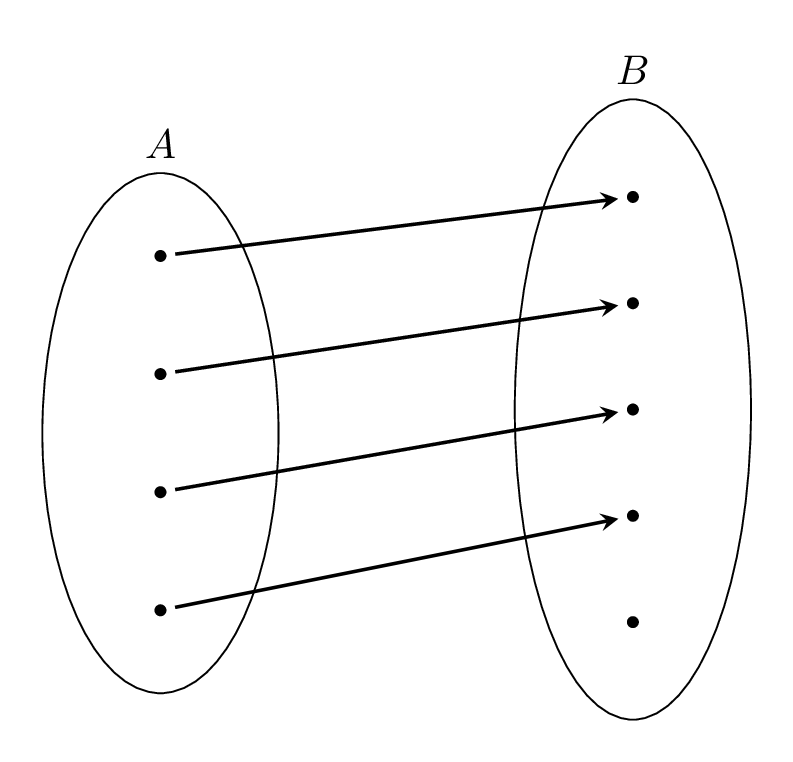
\includegraphics[scale=0.135]{iniettiva}
	\caption{grafico iniettiva}
	\label{fig:grafico_iniettiva}
\end{figure}
\end{defn}
\noindent


\begin{defn} Una funzione si dice \textbf{suriettiva} qunado \textbf{ogni} elemento del codominio è immagine di \textbf{almeno} un elemento del dominio.
\begin{equation}
  b\in B \rightarrow \exists a \in A : f(a) = b
\end{equation}

\begin{figure}[ht]
	\center
	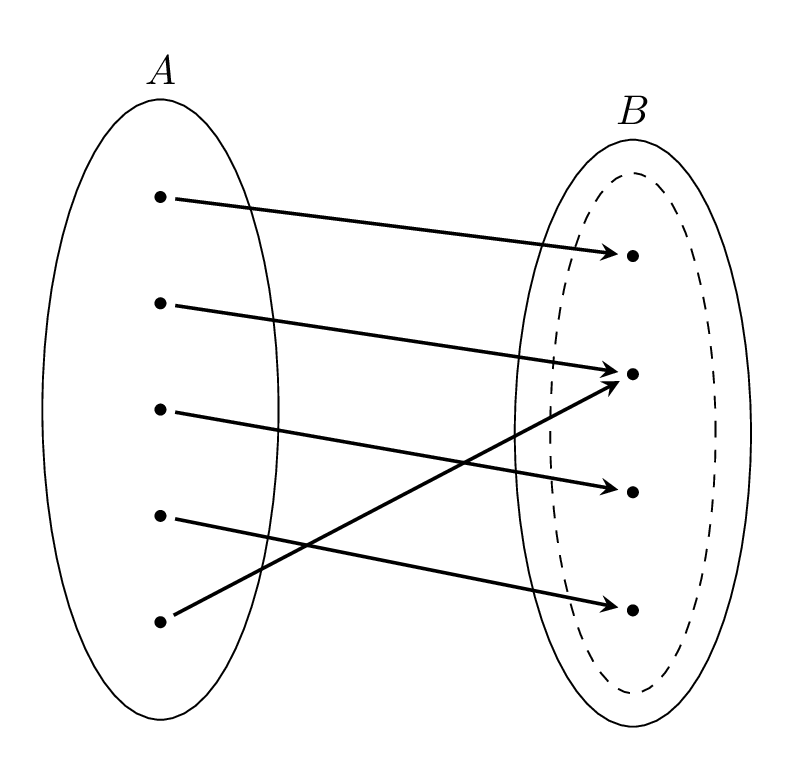
\includegraphics[scale=0.15]{suriettiva}
	\label{fig:grafico_suriettiva}
	\caption{graifco suriettiva}
\end{figure}
\end{defn}


\begin{eser}
Dimostra di che tipo è questa funzione:\vspace{1.5mm}

\begin{equation}
  f :\mathbb{R}\rightarrow \mathbb{R} \qquad f(x)=x^2
\end{equation}

\end{eser}

\begin{dimo}
Non può essere iniettiva perchè per ogni numero reale positivo ne esiste uno uguale negativo, il cui qudrato sarà il \textbf{medesimo}.\vspace{1.5mm}

\begin{equation}
  se\quad x_1 = -x_2 \quad \Rightarrow \quad f(x_1) = f(x_2)
\end{equation}  

\vspace{2mm}
si può provare inoltre che non è una funzione suriettva in quanto \textbf{nessun} numero negativo fa parte del codominio ed esso è formato da $\mathbb{R}$ dunque
\begin{equation}
  -4 \ne f(x) \qquad \forall x \in \mathbb{R}
\end{equation}
\end{dimo}

\begin{eser}
Dimostra di che tipo è questa funzione:
\begin{equation}
  f :\mathbb{N}\rightarrow \mathbb{N} \qquad f(x)=x^2
\end{equation}
\end{eser}

\begin{dimo}
  se cambiamo il dominio e il codominio nell'insieme dei numeri naturali e consideriamo la stessa legge possiamo deddure che:

\begin{equation}
  \forall n,m : n \ne m \quad \Rightarrow \quad n^2 \ne m^2
\end{equation}

\vspace{3.5mm}
Per \textbf{qualsiasi} coppia di numeri naturali diversi fra loro non è possibile pensare che il loro quadrato sia uguale, per tanto la funzione è iniettiva. 
\vspace{2.5mm}
Inoltre \textbf{qualsiasi} numero dispari non avrà una propria immagine, in quanto l'insieme racchiude \textbf{solo} numeri interi positivi. Ovvero:

\begin{equation}
  \exists \frac{x}{2} \in \mathbb{N}: \{y = x + 1\} \quad
  \Rightarrow \quad y \ne n^2 \qquad \forall n\in \mathbb{N}
\end{equation}

\end{dimo}


\subsection{Funzioni invertibili}
\begin{defn} Una funzione $f:A\rightarrow B$ si dice invertibile se esiste una funzione $g: B \rightarrow A$ chiamata funzione inversa tale che:
\begin{itemize}
  \item $\forall a\in A, \quad g(f(a))=a$
  \item $\forall b\in B, \quad f(g(b))=b$
\end{itemize}
Essa si può considerare invertibile se è \textbf{biiettiva}.
\end{defn}

\begin{eser}
  Dimostra se la funzione $f: \mathbb{R} \ \rightarrow \ \mathbb{R} \qquad f(x) = 2x\ +\ 1$ è inversibile.
\end{eser}

\begin{dimo}
Ponendo l'equazione $ y =\ 2x\ +\ 1$ deduciamo che

	\begin{equation}
  		f^{(-1)}(x) = \frac{x\ -\ 1}{2}
	\end{equation}

\vspace{1.5mm}
quindi:
\begin{equation}
  f^{(-1)}(f(x))= f^{(-1)}(2x\ +\ 1)\ = \frac{(2x\ +\ 1)\ -\ 1}{2}\ =\ x;
\end{equation}
\vspace{1.5mm}
e allo stesso tempo

\vspace{1.5mm}
\begin{equation}
f(f^{(-1)}(y))\ = f(\frac{y\ -\ 1}{2})\ +\ 1\ =\ y
\end{equation}
\end{dimo}

\subsection{Piano Cartesiano}
Fissando un'origine e un'unità di misura ad \textbf{ogni} punto di una retta orientata corrisponde uno ed un solo numero reale.
Si stabilisce così una \textbf{corrispondenza biunivoca} tra i punti della retta orientata e i numeri reali.\\
Data la funzione
\vspace{1.5mm}

\begin{equation}
  f: A\ \rightarrow\ B \quad A,B\ \subseteq \mathbb{R}\ \times\ \mathbb{R}\ = \mathbb{R}^2\\
\end{equation}

\begin{figure}[ht]
  \center
  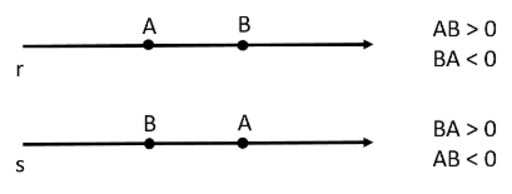
\includegraphics[scale=0.25]{rettaorientata}
  \caption{la retta orientata}
  \label{fig:retta_orientata}
\end{figure}

\begin{defn}
Definiamo una \textbf{coppia} di rette orientate disposte \textbf{perpendicolarmente} fra loro \textbf{assi coordinati}.
\begin{itemize}
  \item{La retta da destra verso sinistra viene chiamata \textbf{asse delle ascisse}}
  \item{la retta dal basso verso l'alto viene chiamata \textbf{asse delle ordinate}}
\end{itemize}
Il punto del piano in cui si incontrano viene chiamato \textbf{origine degli assi} e viene indicato con $O$
\end{defn}

Un qualsiasi punto del piano $P$ viene identificato con una ascissa $x_p$ ed una ordinata $y_p$, quindi $P(x_p, y_p)$.\\
Il piano viene diviso in IV quadranti numerati in senso antiorario.

\begin{figure}[ht]
  \center
  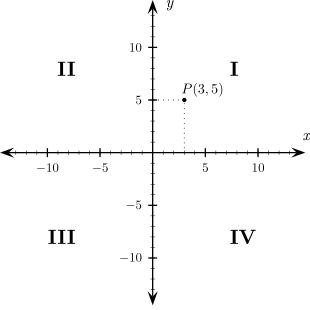
\includegraphics[scale=0.4]{pianocartesiano}
  \caption{il piano cartesiano}
  \label{fig:piano_cartesiano}
\end{figure}

\subsection{Grafici di funzioni}
\raggedright{Ora possiamo rappresentare graficamente coppie ordinate di numeri reali sul piano, quindi possiamo rappresentare il \textbf{grafico} di una funzione}

\begin{equation}
f: A\ \subseteq \mathbb{R}\  \rightarrow \ B \subseteq \mathbb{R}\
\end{equation}\\ \vspace{1.5mm}

e tutte le coppie $(x,\ f(x))$ tali che $x\in A$:\\

\begin{equation}
G(f)\ = \{(x,\ f(x))\} \ :\ x\in A
\end{equation}

\begin{figure}[ht]
  \center
  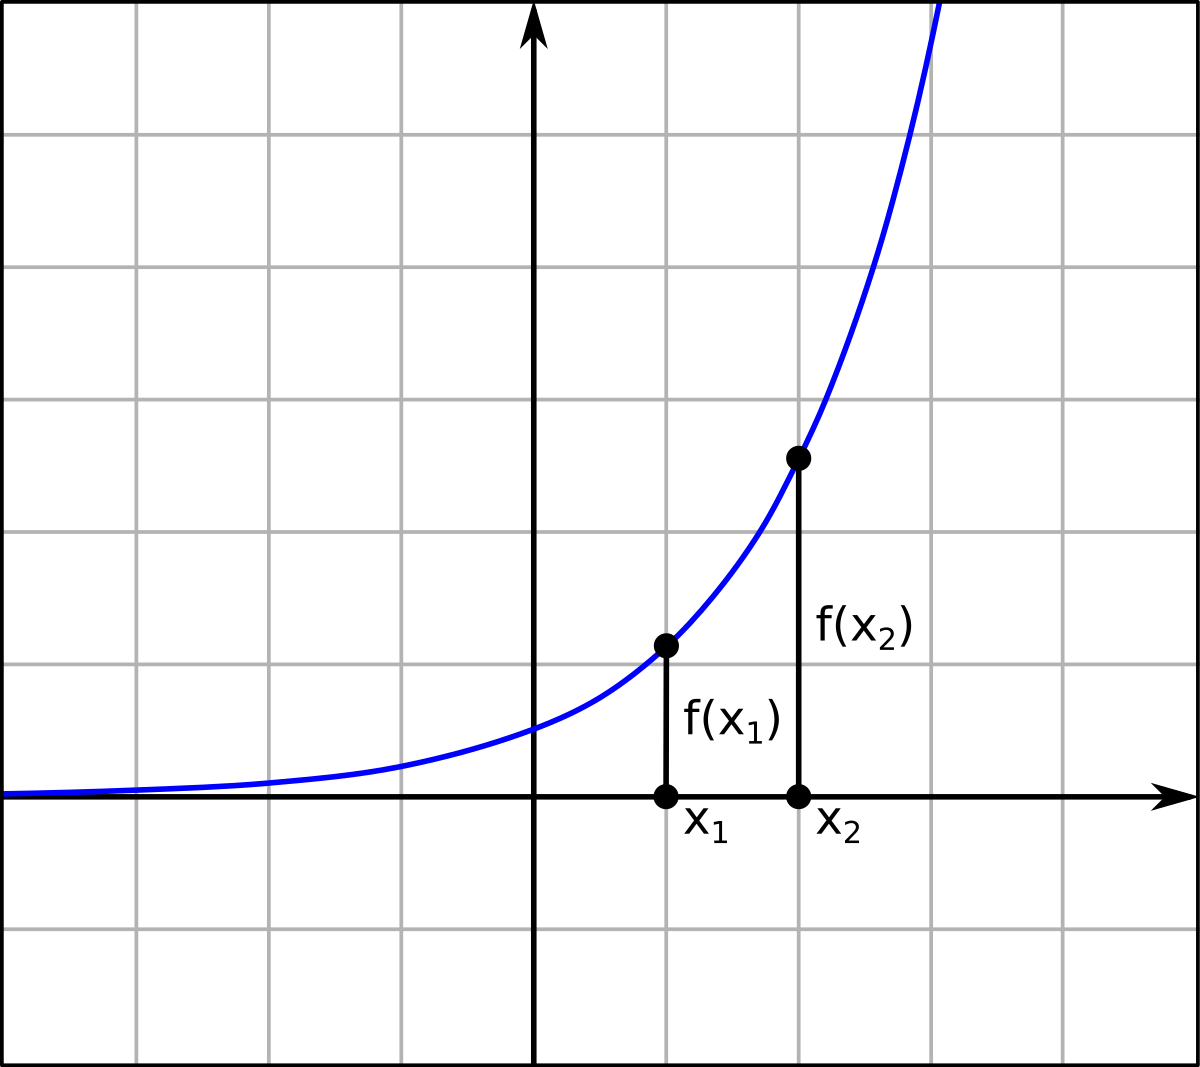
\includegraphics[scale=0.15]{graficofunzione}
  \caption {il grafico di una funzione crescente}
  \label{fig:grafico_funzione}
\end{figure}

\subsection{Funzioni Pari e Dispari}
\begin{defn}
Una funzione $f: [-a, a]\ \rightarrow \ \mathbb{R}$ si dice \textbf{pari} se $f(x) = f(-x)$\\
Si deduce quindi che il grafico di una funzione così definita è simettrico rispetto all'\textbf{asse delle ordinate}
\end{defn}

\begin{figure}
  \center
  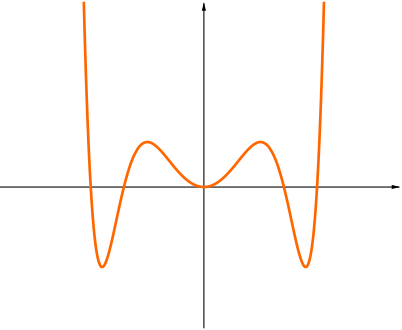
\includegraphics[scale=0.65]{funzionepari}
  \caption{Una funzione pari}
  \label{fig:funzione_pari_grafico}
\end{figure}


\begin{defn}
Una funzione $f: [-a, a]\ \rightarrow \ \mathbb{R}$ si dice \textbf{dispari} se $f(-x) = -f(x)$\\
Si deduce quindi che il grafico di una funzione così definita viene \textbf{specchiata} in due quadranti uno \textbf{oppsoto} all'altro
\end{defn}

\begin{figure}[ht]
  \center
  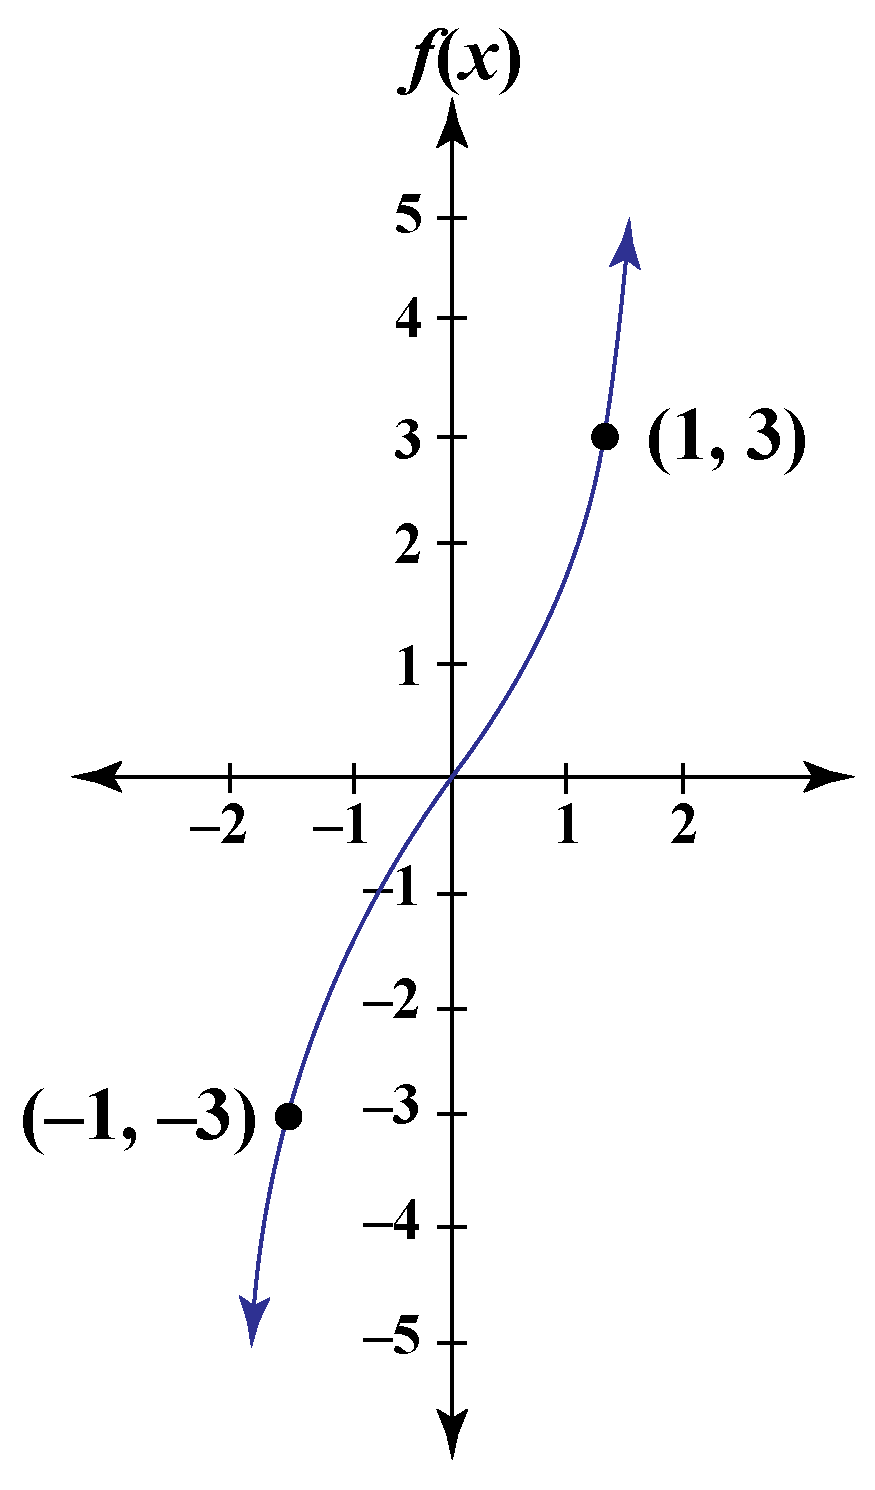
\includegraphics[scale=0.25]{funzionedispari}
  \caption{Una funzione dispari}
  \label{fig:funzione_dispari_grafico}
\end{figure}



\subsection{Funzioni crescenti e decrescenti}
\begin{defn}
 Una funzione $f: [-a, a]\ \rightarrow \ \mathbb{R}$ si dice \textbf{crescente} se
 \begin{equation}
   f(x_2)\ \geq \ f(x_1) \quad \forall x_2 > x_1 \in [a,b]
\end{equation}\\
 Si dice \textbf{strettamente crescente} se\\
 \begin{equation}
  f(x_2)\ \>\ f(x_1) \quad \forall x_2 > x_1 \in [a,b]
\end {equation}


\begin{figure}[ht]
  \center
  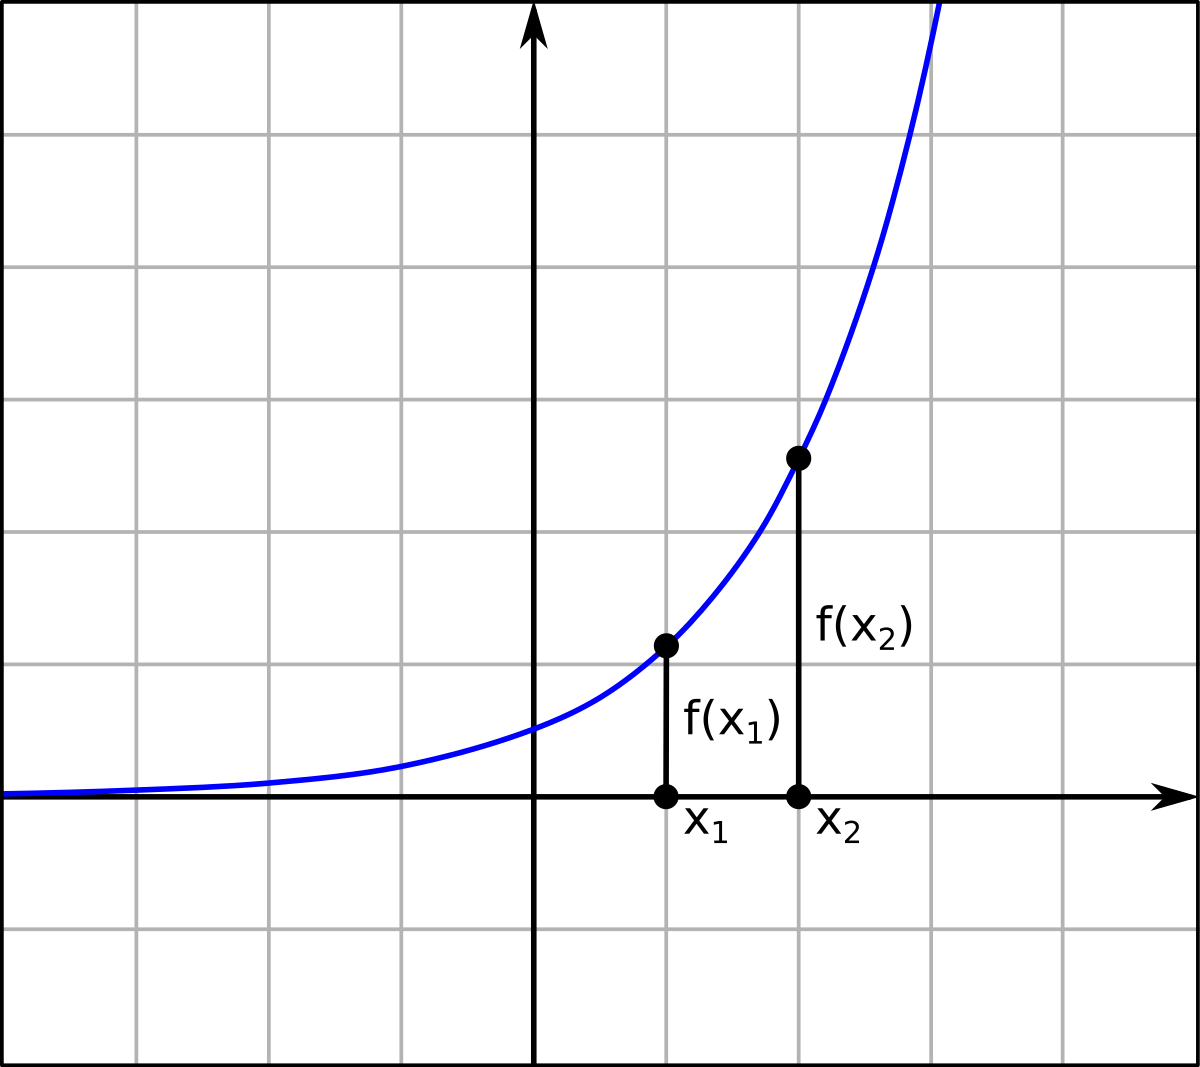
\includegraphics[scale=0.15]{graficofunzione}
  \caption {il grafico di una funzione crescente}
  \label{fig:grafico_funzione_crescente}
\end{figure}

\end{defn}



\begin{defn}
 Una funzione $f: [-a, a]\ \rightarrow \ \mathbb{R}$ si dice \textbf{decrescente} se
 \begin{equation}
   f(x_2)\ \leq \ f(x_1) \quad \forall x_2 > x_1 \in [a,b]
\end{equation}\\
 Si dice \textbf{strettamente decrescente} se\\
 \begin{equation}
  f(x_2)\ <\ f(x_1) \quad \forall x_2 > x_1 \in [a,b]
\end {equation}


\begin{figure}[ht]
  \center
  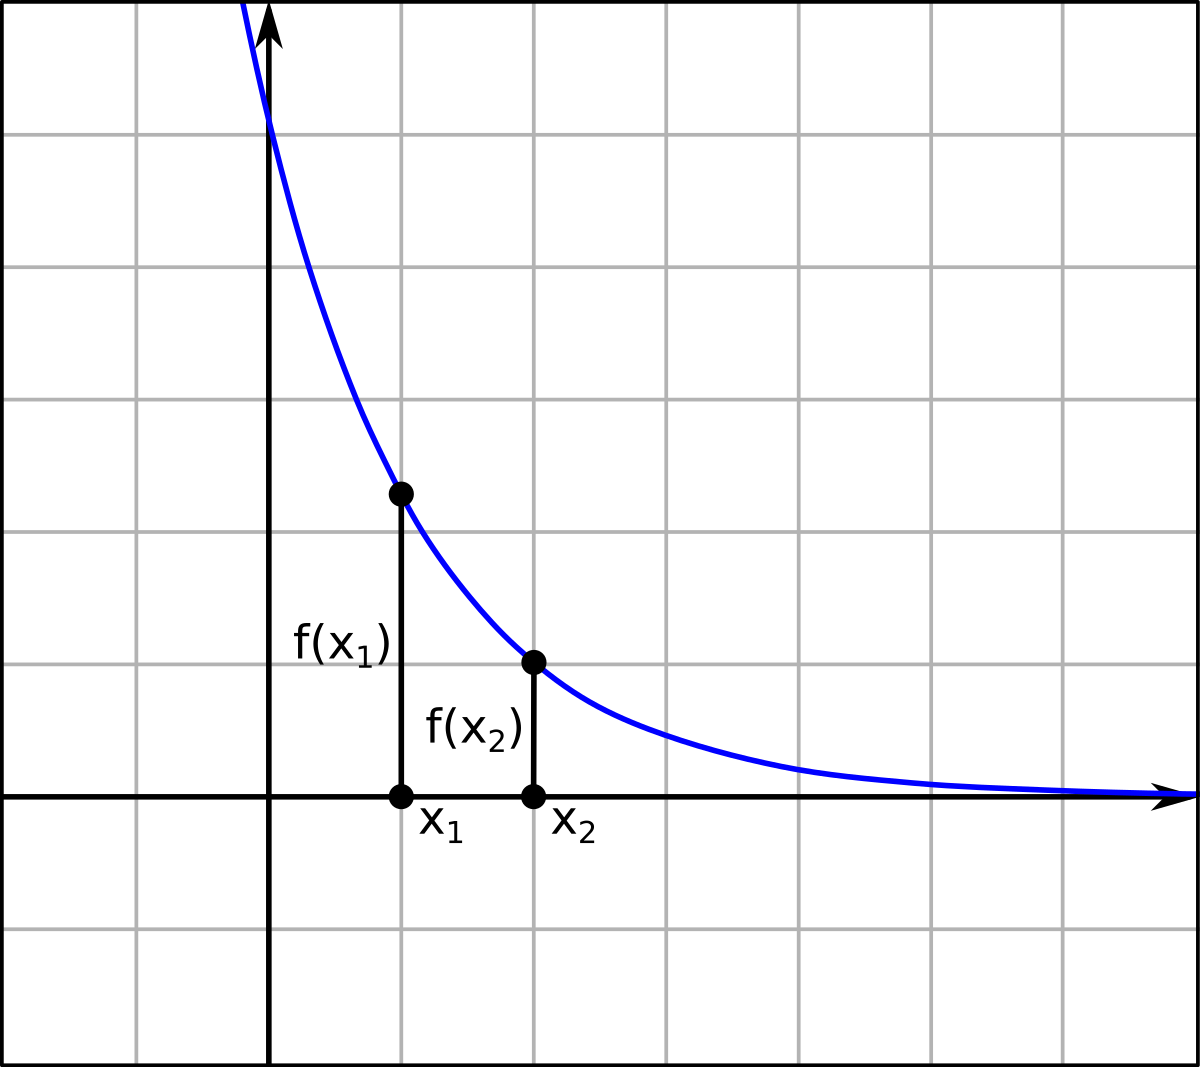
\includegraphics[scale=0.15]{funzionedecrescente}
  \caption {il grafico di una funzione decrescente}
  \label{fig:grafico_funzione_decrescente}
\end{figure}

\end{defn}

\subsection{Funzioni inverse}
Se i punti di una funzione $ f : A\ \rightarrow \ B \quad A,B \subseteq \mathbb{R} $ si ottengono dalle coppie $ (a,b)\in A\ \times\ B $
\begin{defn}
Il grafico di una funzione inversa si ottiene invertendo le coordinate dei punti del grafico. Ovvero i punti del grafico della \textbf{funzione inversa} si ottengono dalle coppie $(b,a)\ \in B\ \times\ A\ $ //
Per via grafica esso può essere ottenuto \textbf{riflettendo} il grafico rispetto alla \textbf{bisettrice} del \textbf{primo} e \textbf{terzo quadrante}

\begin{figure}[ht]
  \centering
  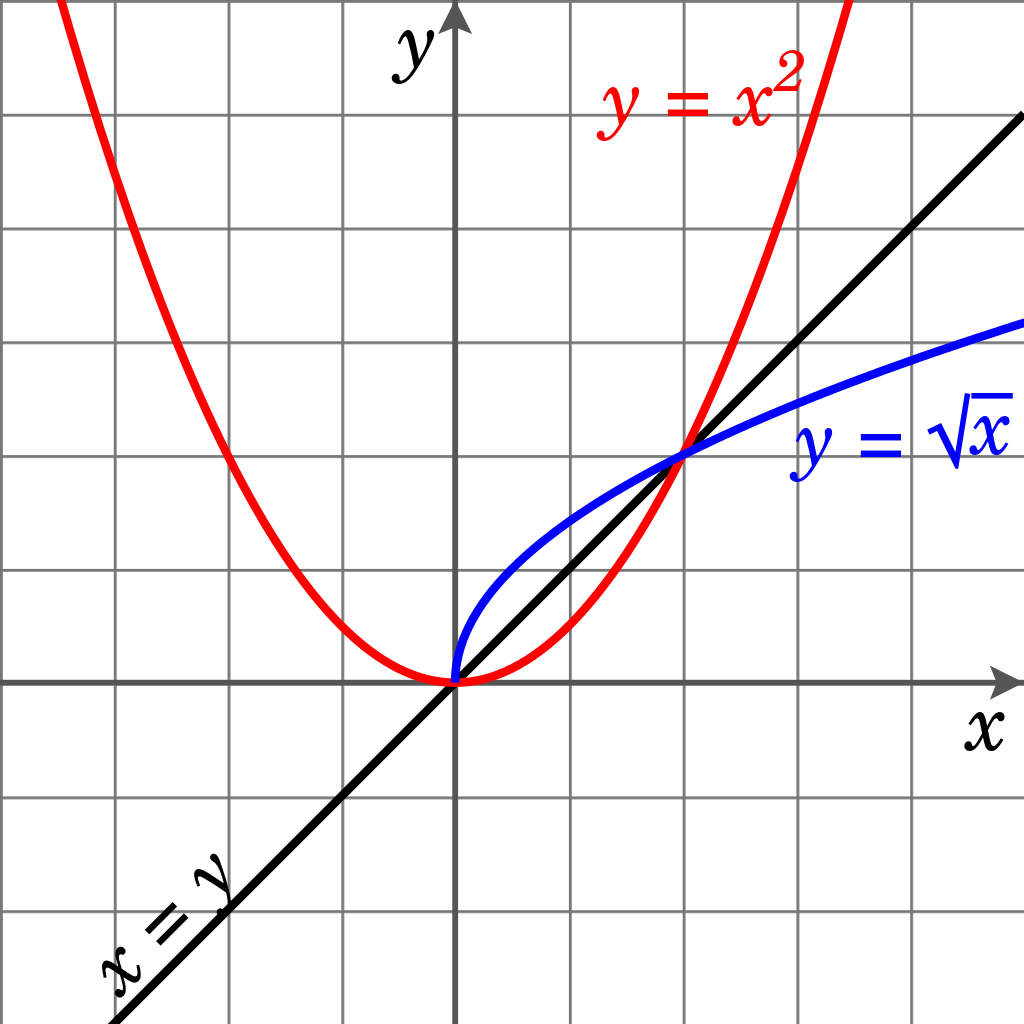
\includegraphics[scale=0.1]{funzioneinversa}
  \caption{Il grafico di una funzione inversa}
  \label{fig:grafico_funzione_inversa}
\end{figure}
\end{defn}

% end of first unit


\subsection{Modelizzazione matematica}

\begin{defn}
  Per \textbf{modelizzazione matematica} si intende un porcesso che ha per scopo quello di \textbf{interpretare} fenomeni legati al mondo reale partendo da dati sperimentali e \textbf{traducendoli} in \textbf{problemi matematici}\\
\end{defn}

Per passare da un fenomeno reale alla sua descrizione mediante modello matematico è necessario un processo di \textbf{astrazione} e \textbf{traduzione} del fenomeno in termini matematici e rigorosi. \\

\vspace{1mm}
Quando si vuole modelizzare un certo fenomeno, si vuole capire \textbf{come} le variabili coinvolte siano in relazione tra loro, ovvero stabilire delle \textbf{leggi matematiche} che descrivono queste relazioni. \\

\vspace{1mm}
La procedura di modelizzazione è:
\begin{enumerate}
  \item si identifica l'incognita del problema
  \item si analizza il fenomeno fisico e si raccolgono informazioni
  \item si individuano le relazioni tra le informazioni raccolte, che poi vengono tradotte in equazioni
  \item si risolvono le equazioni ottenute e se ne verifica la validità del modello
\end{enumerate}


In un modello matematico che coinvolge due grandezze x ed y ci interessa capire come la \textbf{variabile dipendente $(y)$} varia al variare di quella \textbf{indipendente}\\

\begin{esem}
Supponiamo di aver formulato la legge $ y\ =\ f(x)\ $\\
Se il modello è giusto potremmo ricavare il valore di $y$ a partire da qualsiasi valore di $x$ senza effettuare ulteriori esperimenti e misurazioni.\\
Rappresentandolo graficamente:

\begin{figure}[ht]
  \center
  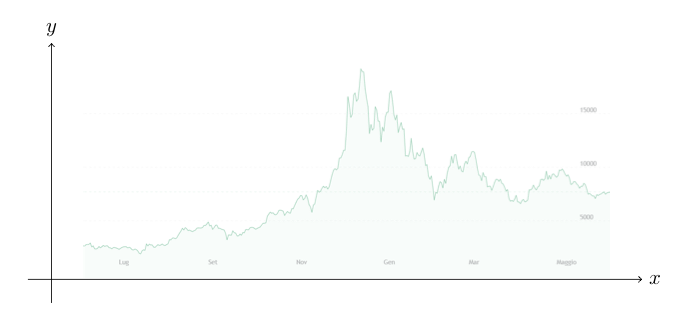
\includegraphics[scale=0.75]{graficobitcoin}
  \caption{Il grafico dell'andamento dei bitcoin}
  \label{fig:btc_chart}
\end{figure}
Questo è il grafico di $y\ =\ f(x)$ dove y="valore del bitcoin in dollari" e x="tempo".
\end{esem}

\subsection{Proporzioni}
\begin{defn}
  Due grandezze $A$ e $B$ si dicono \textbf{direttamente proprozionali} se esiste un numero $c$ detto \textbf{costante di proporzionalità} tale che:

\begin{equation}
  A\ =\ cB
\end{equation}
\end{defn}

Questo significa che le due grandezze sono legate da una certa legge, per la quale quando una raddoppia, triplica, dimezza, di conseguenza la seconda raddoppia, triplica, dimezza etc.

\begin{esem}
  $A$ = "quantità di chilometri che l'auto può percorrere"\\
  $B$ = "litri di carburante nel serbatoio"
\end{esem}

\begin{defn}
  Due grandezze $A$ e $B$ si dicono \textbf{inversamente proprozionali} se esiste un numero $c$ detto \textbf{costante di proporzionalità} tale che:

\begin{equation}
  AB\ =\ c
\end{equation}
\end{defn}
Questo significa che le due grandezze sono tali che all'aumentare di una, l'altra diminuisce proporzionalmente.

\begin{esem}
  $A$ = "numero di partecipanti all'acquisto di un immobile"\\
  $B$ = "quota per partecipante"\\
  $c$ = costo dell'immobile
\end{esem}

\section{Combinatoria e probabilità}
\subsection{Introduzione}

\begin{defn}
  L'\textbf{analisi combinatoria} è la branca della matematica applicata per risolvere problemi nel quale è necessario saper "contare" efficacemente esiti e probabilità di determinate situazioni.\\
  Essa è infatti la disciplina che ci permette di \textbf{contare senza contare}
\end{defn}

\subsection{Combinatoria}
\begin{defn}[Principio di moltiplicazione]
  Un insieme $X$ soddisfa le ipotesi del principio di moltiplicazione se:

  \begin{itemize}
    \item è possibile ottenere ciascuno dei suoi elementi come risultato di una procedura composta da $n$ fasi successive.
    \item se ad una fase interemedia si sono ottenuti due esisti distinti allora la procedura conduce ad elementi distinti di $X$
  \end{itemize}

Nella prima fase avremo $m_1$ possibili esiti nella seconda fase avremo $m_2$ esiti sino alla n-esima fase avremo $m_n$ esiti

\begin{equation}
  |X|\ = m_1\ \times\ m_2\ \times\ ...\ \times\ m_k
\end{equation}
\end{defn}

\begin{eser}
  Calcoliamo il numero di coppie ordinate $(a,b)$ contenenti un numero primo ed uno non primo compresi tra 1 ed 8
\end{eser}

\begin{dimo}
  I numeri primi tra 1 e 8 sono $\{ 2, 3, 5, 7\}$ mentre i numeri non primi tra 1 e 8 sono $\{ 1, 4, 6, 8\}$

\begin{enumerate}[label=\Roman*.]
  \item Scegliamo un qualsiasi elemento di $I_8$: abbiamo 8 possibilità.
  \item Se il primo elemento era primo il secondo non lo sarà, e viceversa se il numero non era primo. In ogni caso avremo 4 distinte possiblità

\end{enumerate}
Il numero di coppie è: $8\ \times\ 4\ =\ 32$
\end{dimo}

\begin{eser}
  Consideriamo un'estrazione in successione di 3 numeri della tombola \textbf{tenendo conto dell'ordine}. Quanti sono i possibili esiti?
\end{eser}

\begin{dimo}
  I numeri della tombola sono 90. Gli scenari possibili sono 2:\\
  Nel primo caso \textbf{senza rimpiazzo} se ogni numero può essere scelto una volta sola, mentre sarà \textbf{con rimpiazzo} se un numero può essere scelto più di una volta.\\

Nel primo caso $(a_1, a_2, a_3)\ :\rightarrow\ (a_1\ \neq\ a_2\ \neq\ a_3\ )$ :

\begin{enumerate}[label=\Roman* \textsc{fase}:]
    \item  $a_1 = 90$
    \item  $a_2 = 90 - 1 = 89$
    \item  $a_3 = 90 - 2 = 88$
\end{enumerate}

Quindi il numero di possibili esiti è:
\begin{equation}
  90\ \times\ 89\ \times\ 88\ =\ 704880
\end{equation}

Nel secondo caso $(a_1,a_2,a_3) :\rightarrow (a_1\ =\ a_2\ =\ a_3)$:
\begin{enumerate}[label=\Roman* \textsc{fase}:]
    \item  $a_1\ =\ 90$
    \item  $a_2\ =\ 90$
    \item  $a_3\ =\ 90$
\end{enumerate}
Quindi il numero di possibili esiti è:

\begin{equation}
  90\ \times\ 90\ \times\ 90\ =\ 90^3\ =\ 729000
\end{equation}
\end{dimo}

\begin{defn}
  Definiamo una regola general per $k$-sequenze di $I_n$.
  Siano $k,n\ \in\ \mathbb{N}$ definiamo $k$-sequenza di $I_n$ una $k$-upla \textbf{ordinata} $(a_1,\ldots ,a_k)$ di elementi \textbf{non necessariamente distinti} di $I_n$ Ovvero:
  \begin{equation}
    (a_1,\ldots,a_k)\in\ \underbrace{I_n\times\ \ldots\ \times\ I_n\ }
  \end{equation}
  % with the command |underbrace or upbrace we can have curly braces up or down a section of a given equation
\end{defn}

Nella definzione di sequenze l'ordine degli elementi della $k$-upla è importante: le 3-sequenze (2, 1 ,3 ) e (3, 1, 2) sono diverse anceh se composte dagli stessi numeri. Vengono comunemente dette \textbf{disposizioni} di \textbf{n} oggetti a $k$ a $k$

\begin{esem}
  Sia $I_4\ =\ {1,2,3,4}$. Allora
  \begin{equation}
    (1,2,3,3,4),\qquad (1,1,1,1,1),\qquad (2,2,1,3,4)
  \end{equation}
  sono 5-sequenze di $I_4$. Invece
  \begin{equation}
    (1,2,3),\qquad (1,1,1),\qquad (2,3,4)
  \end{equation}
  sono 3-sequenze di $I_4$
\end{esem}

\subsection{Fattoriale}

\begin{equation}
  5!=\ 5\ \times\ 4\ \times\ 3\ \times\ 2\ \times\ 1
\end{equation}

\begin{equation}
  n!=
  \begin{cases}
    n\ \times\ (n-1)\ \times\ (n-2)\ \times\ \ldots\ 3\ \times\ 2\
    \times\ 1 &  \mbox{se } n\geq\ 1 \\
    1 &  \mbox{se }n\ =\ 0
  \end{cases}
      % 'cases' is used for system of equations. Write the conditions of the if statements AFTER the & symbol
\end{equation}

\begin{defn}
  Il \textbf{fattoriale} di un numero equivale al prodotto di quel numero per tutti i numeri che lo precedono. I valori dei fattoriale crescono esponenzialmente
  \begin{equation}
    0!=\ 1 \qquad 5!=\ 120 \qquad 6!=\ 720 \qquad 7!=\ 5040 \qquad 10!=\ 3628800
  \end{equation}
\end{defn}

\subsection{Numero di Insiemi}
\begin{defn}
	Il \textbf{numero di sottoinsiemi} di $k$ elementi di $I_n$ si distinguono esclusivamente dagli elementi di cui fanno parte: \textbf{l'ordine non conta}.
\end{defn}

Spesso un sottoinsieme di $k$ elementi di un insieme di $n$ elementi viene chiamato \textbf{combinazione} (semplice, senza ripetizioni) di $n$ elementi a $k$ a $k$

\begin{defn}
	Siano $k,n \in \mathbb{N}$ il \textbf{binomiale} di $n$ su $k$ è:
	\begin{equation}
		\bfrac{n}{k}\ =
		\begin{cases}
			\frac{n!}{k!(n-k)!}, & \mbox{se} k\ \leq\ n,\\
			0, 		    & \mbox{se} k\ > n.
		\end{cases}
	\end{equation}
	Il numero di sottoinsiemi di $k$ elementi di $I_n$ è 
	\begin{equation}
		\bfrac{n}{k}.
	\end{equation}
\end{defn}


\begin{esem}
	Calcola i sotttoinsiemi con $3$ elementi di $I_6$
\end{esem}

\begin{dimo}
	La soluzione è data da una semplice applicazione della formula prima vista:
	\begin{equation}
		\bfrac{6}{3}\ =\ \frac{6!}{3!3!}\ =\ 20
	\end{equation}
\end{dimo}


\begin{esem}
	Calcola il numero di partite giocate nella fase a gironi dei Mondiali di calcio. Ci sono 3$2$ squadre divise in $8$ gironi da $4$ squadre ed in ogni girone una squadra deve giocare contro le altre una volta sola.
\end{esem}

\begin{dimo}
	Il numero di partite totale è $8$ volte le partite giocate in un singolo girone.
	L'insieme delle 4 squadre in un girone possiamo identificarlo con $I_4$, e una partita tra 2 squadre con un sottoinsieme di $2$ elementi di $I_4$. Il numero di partite giocate in un girone\textbf{è il numero di sottoinsiemi} di $2$ elementi di $I_4$ ovvero:
	\begin{equation}
		\bfrac{4}{2}\ =\ \frac{4!}{2!(4-2)! }\ =\ \frac{4\times 3\times 2\times 1}{2\times 2}\ = \frac{24}{4}\ =\ 6
	\end{equation}
	Infine il risultato equivale a: $ 6 \times 8 = 48$
\end{dimo}





\end{document}
